\documentclass[10pt, a4paper]{article}
\usepackage{lrec2006}
\usepackage{graphicx}

\usepackage[utf8]{inputenc}

\usepackage{alltt}  
\usepackage{tabularx}  
\usepackage{tipa}  

\usepackage{url}
%\usepackage{natbib}

%\newcommand{\mytexttt}[1]{\texttt{\textscale{0.9}{#1}}}

%\definecolor{MyGray}{rgb}{0.90,0.90,0.90}
%\makeatletter\newenvironment{graybox}{%
%   \begin{lrbox}{\@tempboxa}\begin{minipage}{.98\textwidth}}{\end{minipage}\end{lrbox}%
%   \colorbox{MyGray}{\usebox{\@tempboxa}}
%}\makeatother


\title{Dbnary: Wiktionary as Linked Data for 12 Language Editions with Enhanced Translation Relations}

\name{Gilles Sérasset, Andon Tchechmedjiev}

\address{Univ. Grenoble Alpes, LIG, F-38000 Grenoble, France\\
CNRS, LIG, F-38000 Grenoble, France\\ 
\texttt{firstname.lastname@imag.fr}}

\abstract{ 
This paper presents the current state of development of the DBnary dataset. DBnary is a RDF dataset, structured using the LEMON vocabulary, that is extracted from twelve different Wiktionary language editions. DBnary also contains additional relations from translation pairs to their source word senses.
The extracted data is registered at \url{http://thedatahub.org/dataset/dbnary}.\\ \newline
\Keywords{Wiktionary, Multilingual Lexical Resource, Lexical Networks, LEMON, RDF}}

\date{}

\begin{document}

\maketitleabstract

\section{Introduction}

The GETALP (Study group for speech and language translation/processing) team of the LIG (Laboratoire d'Informatique de Grenoble) is in need for multilingual lexical resources that should include language correspondences (translations) and word sense definitions. In this regard, the set data included in the different Wiktionary language edition is a precious mine.

Alas, many inconsistencies, errors, difference in usage do exist in the various Wiktionary language edition. Hence, we decided to provide an effort to extract precious data from this source and provide it to the community a Linked Data. This dataset won the Monnet Challenge in 2012, when it consisted of 6 language editions. The structure of this dataset, which is intensively based on the LEMON model \cite{Mccrae:2012:ILR:2423739.2423818} is presented in \cite{serasset:dbnary-swj}. This short paper purpose is to present the current state of our dataset.

\section{Extracting Data from Wiktionary}

\subsection{No Common Approach}

Errors and incoherences are inherent to a contributive resource like Wiktionary. This has been heavily emphasized in related works by \cite{HellmannSebastianandBrekleJonasandAuer} and \cite{TUD-CS-2012-0008}. Still, we suceeded not only in extracting data from 12 different language editions, but we are maintaining these extractor on a regular basis. Indeed, our dataset evolves along with the original Wiktionary data. Each time a new Wiktionary dump is available (about once every 10/15 days for each language edition), the DBnary dataset is updated. This leads to a different dataset almost every day.

Some language editions (like French and English) have many moderators that do limit the number of incoherence among entries of the same language. Moreover, those languages that contain the most data, use many \textit{templates} that simplify the extraction process. For instance, the translation section of the French dictionary usually uses a template to identify each individual translation.

This is not true however, with less developed Wiktionary language editions. For instance, in the Finnish edition, some translations are introduced by a template giving the language (e.g. \{fr\} precedes French translation) and others are introduced by the string "ranska" which is the Finnish translation for "French". In this case the translator needs to know the Finnish translation of all language names to cope with the second case and avoid losing almost half of the available translation data.

Moreover, since 2012, we have added new languages that exhibits a different use of the Wikimedia syntax. For instance, translations in the Russian Wiktionary are entirely contained in one unique template, where target languages are a parameter. Moreover, in the Bulgarian Wiktionary, the full lexical entry is contained in one single template where sections are the parameters. In such language editions, templates can not be parsed using regular expressions, as they are inherently recursive (template calls are included in parameter values of other templates). This invalidates our initial approach which was based on regular expressions. In order to cope with these languages, we had to use an advanced parser of the Wikimedia syntax (called Bliki engine\footnote{\url{https://code.google.com/p/gwtwiki/}}) to deal with such data.

Our extractors are written in Java and are open-source (LGPL licensed, available at \url{http://dbnary.forge.imag.fr}).


\begin{figure*}[htb]
	\begin{center}
		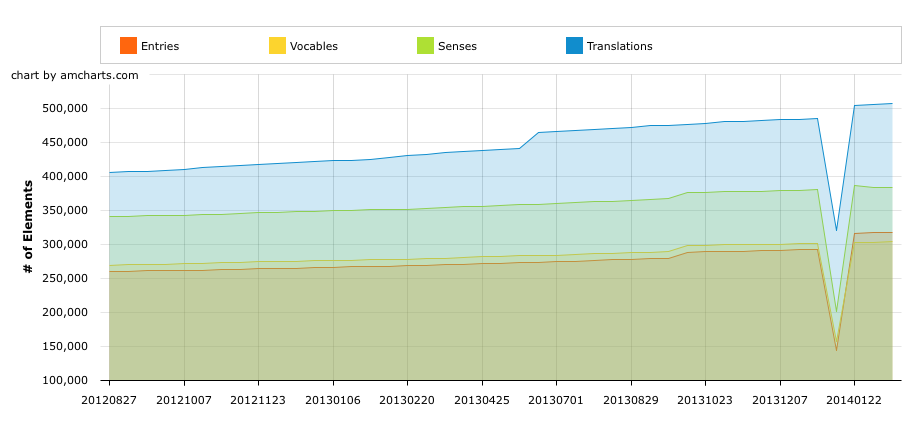
\includegraphics[width=\textwidth]{french.png}
	\end{center}
	\caption{Some of the statistics available about the French extracted data.}
	\label{fig:french}
\end{figure*}

\begin{table*}[hbt]
\begin{minipage}{\linewidth}
\begin{center}
\begin{small}
\begin{tabular}{lrrrrrr}
\hline
\textbf{Language} & Entries & Vocables & Senses & Translations & $\mathbf{Total}$ \\
\textbf{Bulgarian} & $18,831$ & $27,071$ & $18,798$ & $13,888$ & $\mathbf{78,588}$ \\
\textbf{English} & $553,499$ & $528,341$ & $447,073$ & $1,332,332$ & $\mathbf{2,861,245}$ \\
\textbf{Finnish} & $50,813$ & $50,488$ & $59,612$ & $122,724$ & $\mathbf{283,637}$ \\
\textbf{French} & $318,101$ & $304,465$ & $383,242$ & $507,359$ & $\mathbf{1,513,167}$ \\
\textbf{German} & $211,564$ & $282,902$ & $102,468$ & $390,938$ & $\mathbf{987,872}$ \\
\textbf{Italian} & $34,363$ & $101,525$ & $45,022$ & $62,305$ & $\mathbf{243,215}$ \\
\textbf{Japanese} & $25,492$ & $25,637$ & $29,679$ & $87,906$ & $\mathbf{168,714}$ \\
\textbf{Modern Greek (1453-)} & $246,211$ & $241,845$ & $137,072$ & $57,615$ & $\mathbf{682,743}$ \\
\textbf{Portuguese} & $45,788$ & $45,968$ & $81,807$ & $267,801$ & $\mathbf{441,364}$ \\
\textbf{Russian} & $130,879$ & $143,653$ & $116,925$ & $365,389$ & $\mathbf{756,846}$ \\
\textbf{Spanish} & $58,679$ & $65,854$ & $85,852$ & $114,951$ & $\mathbf{325,336}$ \\
\textbf{Turkish} & $64,899$ & $69,383$ & $91,418$ & $66,928$ & $\mathbf{292,628}$ \\
\textbf{Total} & $\mathbf{1,759,119}$ & $\mathbf{1,887,132}$ & $\mathbf{1,598,968}$ & $\mathbf{3,390,136}$ & $\mathbf{8,635,355}$ \\
\end{tabular}
\end{small}
\end{center}
\end{minipage}
\caption{Number of lexical elements in the graphs.}
\label{table:size}
\end{table*}

\begin{table*}[htb]
\begin{center}
\begin{small}
\begin{tabular}{lrrrrrrrr}
\hline
\textbf{Language} & $syn$ & $qsyn$ & $ant$ & $hyper$ & $hypo$ & $mero$ & $holo$ & $\mathbf{Total}$ \\
\textbf{Bulgarian} & $17632$ & $0$ & $34$ & $0$ & $0$ & $0$ & $0$ & $\mathbf{17666}$ \\
\textbf{English} & $31762$ & $0$ & $6980$ & $1252$ & $1212$ & $112$ & $0$ & $\mathbf{41318}$ \\
\textbf{Finnish} & $2478$ & $0$ & $0$ & $0$ & $0$ & $0$ & $0$ & $\mathbf{2478}$ \\
\textbf{French} & $31655$ & $2133$ & $6879$ & $9402$ & $3739$ & $970$ & $1898$ & $\mathbf{56676}$ \\
\textbf{German} & $29288$ & $0$ & $15079$ & $33251$ & $10413$ & $0$ & $0$ & $\mathbf{88031}$ \\
\textbf{Italian} & $9662$ & $0$ & $3425$ & $0$ & $0$ & $0$ & $0$ & $\mathbf{13087}$ \\
\textbf{Japanese} & $3828$ & $0$ & $1578$ & $9$ & $14$ & $0$ & $0$ & $\mathbf{5429}$ \\
\textbf{Greek} & $4990$ & $0$ & $1428$ & $0$ & $0$ & $0$ & $0$ & $\mathbf{6418}$ \\
\textbf{Portuguese} & $3350$ & $0$ & $556$ & $6$ & $4$ & $0$ & $0$ & $\mathbf{3916}$ \\
\textbf{Russian} & $24941$ & $0$ & $9888$ & $22832$ & $5140$ & $0$ & $0$ & $\mathbf{62801}$ \\
\textbf{Spanish} & $15087$ & $0$ & $1525$ & $741$ & $560$ & $0$ & $0$ & $\mathbf{17913}$ \\
\textbf{Turkish} & $3260$ & $0$ & $220$ & $483$ & $164$ & $0$ & $0$ & $\mathbf{4127}$ \\
\textbf{Total} & $\mathbf{177933}$ & $\mathbf{2133}$ & $\mathbf{47592}$ & $\mathbf{67976}$ & $\mathbf{21246}$ & $\mathbf{1082}$ & $\mathbf{1898}$ & $\mathbf{319860}$ \\
\end{tabular}
\end{small}
\end{center}
\caption{Number of lexico-semantic relations in the graphs.}
\label{table:rels}
\end{table*}

\subsection{Tools to Help Maintenance}

In this effort, we also had to develop tools to evaluate the extarctor's performance and to maintain it. Our first tool\footnote{this heuristic was initially suggested by Sebastian Hellman} compares extracted translations with interwiki links. Many of the translations in a Wiktionary language edition do point to entries in the Wiktionary edition of the target language. Such inter-wiki links are available through the Wiktionary API. By randomly sampling the extracted data, we are able to compare the extracted data with such links. This gives us an idea of the extractor performance. However, this relies on the availability of inter-wiki links, which is not the case in some language edition.

When we maintain the extractor, we need to carefully check that the patches we added do not introduce regressions in the extractor. For this, we developped our own \texttt{RDFdiff} command line tool which computes the differences between 2 RDF dumps. Such a command is already provided in the JENA toolbox, however, the JENA implementation does not correctly deal with anonymous nodes. Indeed, anonymous nodes are always considered as different by the JENA implementation when the RDF specification states that 2 anonymous nodes that share the same properties should be considered equal. Our version of RDFDiff correctly handles such anonymous node (that are heavily used in the LEMON model). With this implementation, it is now easy to compute the difference between the original extraction and the new one and to decide, based on these differences, if the new version is good enough for production.

From time to time, a Wiktionary language edition drastically changes the way it encodes some data. Actively following the discussions on each Wiktionary edition to anticipate such changes is not an option with so many languages. Hence, with each language extraction update, we compute a set of statistics that gives detailed figures on the size of the data . These statistics are available live on the DBnary web site\footnote{\url{http://kaiko.getalp.org/about-dbnary}}. Overall, the most useful statistics are the ones that capture the evolution of the extracted data over time. For instance Figure \ref{fig:french} shows the evolution of the size of the extracted French datasets since its original extraction. This plot allowed us to detect that a major refactoring was happening on the French language edition. This allowed us to patch the extractor for this new organisation right away.

\section{Extracted Data as a LEMON Lexical Resource}

\subsection{Extracted Entries}

The main goal of our efforts is not to extensively reflect the specific structures and constructs of Wiktionary data, but to create a lexical resource that is structured as a set of monolingual dictionaries + bilingual translation information. Such data is already useful for several application, but most importantly it is a sound starting point for a future multilingual lexical database.

Monolingual data is always extracted from its dedicated Wiktionary language edition. For instance, the French lexical data is extracted from the French language edition (the data is available on http://fr.wiktionary.org). However, we do not capture as of yet, any of the French data that may be found in other language editions.

We also filtered out some parts of speech in order to produce a result that is closer to existing monolingual dictionaries. For instance, in French, we disregard abstract entries corresponding to prefixes, suffixes or flexions (e.g.: we do not extract data concerning \textit{in-} or \textit{-al} that are prefixes/suffixes and that have a dedicated page in the French language Edition). 

Given that the scope and main focus of our work is the production of lexical data, we do not provide any reference or alignment to any ontology (toward top-level concepts for example).  



\subsection{LEMON and non-LEMON modelled Extracted Data}

All of the extracted data could not be structured using solely the LEMON model. For instance, LEMON does not contain any mechanisms that allow to represent translations between languages, as the underlying assumption is that such translation will be handled by the ontology description. Moreover, LEMON further assumes that all data is well-formed and fully specified. As an example, the synonymy relation is a property linking a \textit{Lexical Sense} to another \textit{Lexical Sense}. While this is a correct assumption in \textit{principle}, it does not account for the huge amount of legacy data that is available in dictionaries and lexical databases and that isn't disambiguated.

In order to cope with such legacy data, we introduced several classes and properties that are not LEMON entities. However, we make sure that whenever a piece of data can be represented as a LEMON entity, it is indeed represented as such. Most of these points have already been covered in \cite{serasset:dbnary-swj}.


\subsection{Links to other datasets}

The DBnary dataset makes use of other datasets. Firstly, while all extracted lexical entries are associated with a language-specific part of speech that is given by its original Wiktionary language edition, we also add, when available a \texttt{lexinfo:partOfSpeech} relation to a standard value defined in the \textit{LexInfo} ontology\footnote{\url{http://www.lexinfo.net/ontology/2.0/lexinfo}} \cite{Lexinfo}. Secondly, while the LEMON model uses a string value to represent languages, we additionally use the property \texttt{dcterms:lang} to point to a language entity defined in the \emph{Lexvo} ontology \cite{deMeloWeikum2008c}.

\subsection{Disambiguation of translation sources}

Many of the translations present in Wiktionary are associated with a hint used by human users to identify the sense of the source of the translation. Depending on the language, this hint may take the form of a sense number (e.g. in German and Turkish), of a textual gloss (e.g. English) or of both a sense number and a textual gloss (e.g. French, Finnish).

By using an adaptation of various textual and semantic similarity techniques based on partial or fuzzy gloss overlaps, we were able to disambiguate the translation relations. We obtained F-measures of the order of 80\% (on par with similar work on English only, such as \cite{meyer-gurevych:2012:PAPERS}), across the three languages where we could generate a gold standard (French, Portuguese, Finnish). We have shown that most of the disambiguation errors are due to inconsistencies in Wiktionary itself that cannot be detected at the generation of DBnary (shifted sense numbers, inconsistent glosses, etc.).  

The relations between translations and lexical senses has also been made part of this dataset.

\subsection{Size of the involved data}

 Table~\ref{table:size} gives an overview of the number of main elements (Entries, Vocables, Senses and Translation), as extracted from the most up-to-date dumps at the time of writing. Table~\ref{table:rels} details the number of lexico-semantic relations contained in each extracted languages.



\section{Conclusion and Perspectives}

The present article exhibits some preliminary results on what is essentially an open source tool to extract a LEMON based lexical network from various Wiktionary language editions. Such a work is interesting for many users that will be able to use the extracted data in their own NLP systems. Moreover, as the extracted resource uses the Resource Description Framework (RDF) standard and the LEMON model, the extracted data is also directly usable for researchers in the field of the Semantic Web, where it could be used to ease the construction of ontology alignment systems when terms in different languages are used to describe the ontologies of a domain.

Current work consists in extending the set of extracted languages, generalizing the extraction engine so that maitenance and definition of extractors will be easier, and adding more semantics to the dataset by providing internal and external links to \textit{LexicalSenses} (as we started with translations). We are currently working on cross-lingual string similarity measures that will be used to establish such links.

Also, we believe that the different initiatives aiming the extraction of Lexical Data from Wiktionary (e.g. UBY \cite{TUD-CS-2012-0008} or \cite{HellmannSebastianandBrekleJonasandAuer}), should meet and work conjointely to produce even better and larger Lexical Linked Data.

\section{Acknowledgements}

This work was conducted as a part of the CHIST-ERA CAMOMILE project, which was funded by the ANR (Agence Nationale de la Recherche, France).

\bibliographystyle{lrec2006}      % basic style, author-year citations
\bibliography{biblio}   % name your BibTeX data base

%\nocite{*}
\end{document}

